\section{Erstellung des Sechobjects}

\begin{figure}[h]
	\centering
	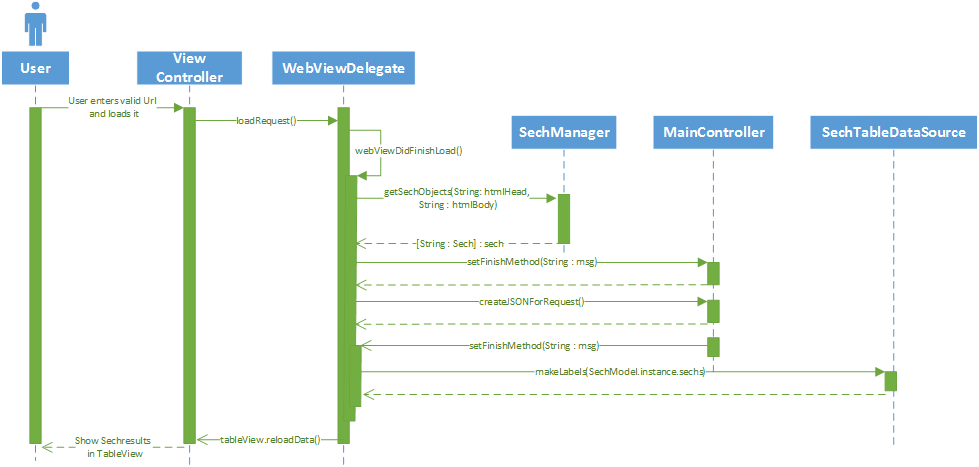
\includegraphics[scale=0.6]{sechobject.png}
	\caption{Ablauf der Erstellung eines \SECH-Objektes}
	\label{fig:SECH-Objekt Erstellung}
\end{figure}

Sobald der User eine gültige URL eingibt und lädt, wird die Laderoutine \Verb|loadRequest()|
angestoßen. Ist die Seite fertig geladen wird in der Delegatemethode \Verb|webViewDidFinishLoad()|
des WebViewDelegates das Auslesen bzw. Laden der \SEARCH-Tags begonnen.

Dem \SEARCH-Manager wird der HTML-Head und Body der eben geladenen Website übergeben und es
werden mit Hilfe des HTMLManagers \SEARCH-Objekte erstellt. Diese \SEARCH-Objekte werden in einem
Dictionary zurückgegeben.

Sobald ein \SECH-Object-Dictionary zurückgegeben wurde, werden die Ergebnisse gerankt und an den SechTableDataSource übergeben. Anschließend wird mit reloadData() die Tabelle der \SECH-Tags im ViewController befüllt.
